\documentclass[12pt,a4paper,UTF8]{ctexart}
\usepackage{geometry}
\geometry{left=2.5cm,right=2.5cm,top=2.8cm,bottom=2.5cm}
\usepackage{graphicx}
\usepackage{amsmath,amssymb}
\usepackage{array}
\usepackage{multirow}
\usepackage{makecell}
\usepackage{booktabs}
\usepackage{caption}
\usepackage{float}
\usepackage{fancyhdr}
\usepackage{setspace}
\usepackage{enumitem}

% 全局行距与段落
\onehalfspacing
\setlength{\parindent}{0pt}
\setlength{\parskip}{6pt}

% 页眉页脚
\setlength{\headheight}{15pt}
\pagestyle{fancy}
\fancyhf{}
\fancyhead[C]{\small \bfseries 哈尔滨工业大学（深圳）实验报告}
\fancyfoot[C]{\thepage}
\renewcommand{\headrulewidth}{0.5pt}
\renewcommand{\footrulewidth}{0pt}

% 公式间距
\setlength{\abovedisplayskip}{10pt}
\setlength{\belowdisplayskip}{10pt}

% 列表优化
\setlist[enumerate]{itemsep=0.5em, topsep=0.5em}

\begin{document}

% 封面
\begin{titlepage}
    \centering
    \vspace*{1cm}
    
\includegraphics[width=0.22\textwidth]{logo.png}\\[0.6cm]
    \Huge\bfseries 哈尔滨工业大学（深圳）\\[0.3cm]
    \normalsize Harbin Institute of Technology, Shenzhen\\[2.2cm]
    \Huge\bfseries 实验报告\\[0.3cm]
    \rule{\linewidth}{0.5mm}\\[3.2cm]
    
    \Large
    \renewcommand{\arraystretch}{1.4}
    \begin{tabular}{ll}
        课程名称： & 自动控制理论 \\
        学生姓名： & 余泓彬 \\
        班级学号： & 2024312506 \\
        学生专业： & 电气工程及其自动化 \\
        实验名称： & 实验二 典型系统的时域响应和稳定性分析 \\
        报告时间： & \today
    \end{tabular}
    
    \vfill
    \Large 哈尔滨工业大学（深圳）
\end{titlepage}

\section{实验二 典型系统的时域响应和稳定性分析}
\hrule

\subsection{预习要求}
1. 预习实验内容，完成表达式及部分参数计算。
2. 实验步骤、数据处理过程写在实验报告中。
3. 依据实际实验结果结合理论分析并回答思考题内容。

\subsection{一、实验目的}
\begin{enumerate}[leftmargin=*]
    \item 分析二阶系统特征参数 $\xi$、$\omega_n$ 对系统动态性能的影响。
    \item 学习使用 Routh 判据对三阶系统进行稳定性判断。
    \item 掌握二阶系统时域性能指标的测试与计算方法。
    \item 通过实验验证理论分析结果，加深对系统响应与稳定性的理解。
\end{enumerate}

\subsection{二、实验设备及元器件}
\begin{enumerate}[leftmargin=*]
    \item PC 计算机
    \item NI ELVIS III 实验平台
    \item 自动控制原理实验套件（Circuits Control Board - 1）
    \item 连接导线若干
\end{enumerate}

\subsection{三、实验原理}
本实验围绕典型二阶、三阶系统展开，通过模拟电路与理论计算，分析系统时域响应、稳定性及极点分布规律。

\subsubsection{3.1 典型二阶系统动态性能分析}
(1) 系统框图
\begin{figure}[H]
    \centering
    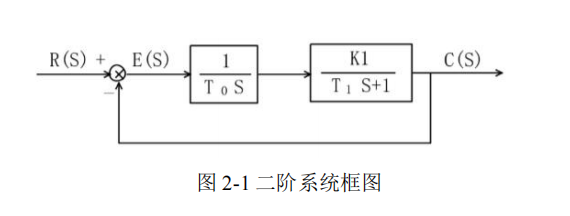
\includegraphics[width=0.7\textwidth]{2.1.png}
    \caption{典型二阶系统框图}
\end{figure}

(2) 模拟电路图
\begin{figure}[H]
    \centering
    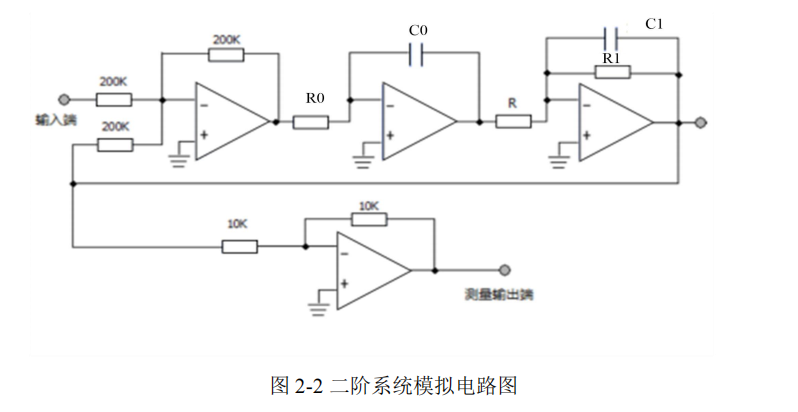
\includegraphics[width=0.7\textwidth]{2.2.png}
    \caption{典型二阶系统模拟电路}
\end{figure}

系统开环传递函数：
\[
G(s)=\frac{K_1}{T_0 s(T_1 s + 1)}
\]
系统闭环传递函数：
\[
\Phi(s)=\frac{\omega_n^2}{s^2+2\xi\omega_n s+\omega_n^2}
\]

\textbf{推导 $T_0$、$T_1$、$K_1$ 的表达式}
\[
T_0=R_0C_0,\quad T_1=R_1C_1,\quad K_1=\frac{R_0}{R}
\]

\textbf{推导求出特征参量 $\xi$、$\omega_n$ 表达式}
\[
\omega_n=\frac{1}{\sqrt{T_0 T_1}},\quad 
\xi=\frac{T_0+T_1}{2\sqrt{T_0 T_1}}
\]
代入参数：$R_0=500\ \mathrm{k}\Omega$，$C_0=2\ \mathrm{\mu F}$，$R_1=200\ \mathrm{k}\Omega$，$C_1=1\ \mathrm{\mu F}$
\[
T_0=1\ \mathrm{s},\quad T_1=0.2\ \mathrm{s}
\]
\[
\omega_n=\sqrt{5}\approx2.236\ \mathrm{rad/s},\quad \xi\approx0.671
\]

\newpage
\subsubsection{3.2 利用 Routh 判据分析典型三阶系统稳定性}
(1) 三阶系统框图
\begin{figure}[H]
    \centering
    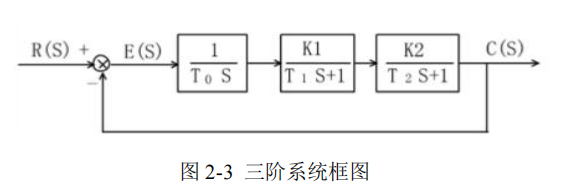
\includegraphics[width=0.7\textwidth]{2.3.png}
    \caption{典型三阶系统框图}
\end{figure}

(2) 三阶系统模拟电路图
\begin{figure}[H]
    \centering
    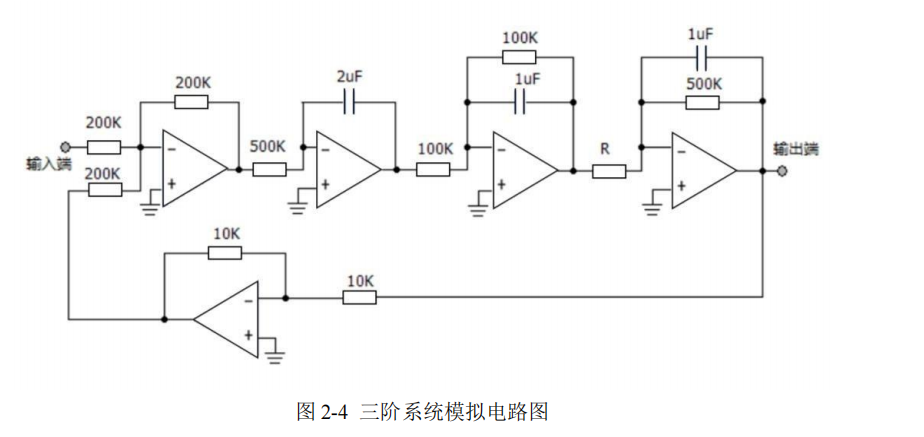
\includegraphics[width=0.7\textwidth]{2.4.png}
    \caption{典型三阶系统模拟电路}
\end{figure}

系统开环传递函数：
\[
G(s)=\frac{K}{s(s+2)(s+10)}
\]
系统特征方程：
\[
s^3 + 12s^2 + 20s + 20K = 0
\]

\textbf{由 Routh 判据得到 Routh 行列式为：}
\begin{table}[H]
\centering
\renewcommand{\arraystretch}{1.5}
\setlength{\tabcolsep}{30pt}
\begin{tabular}{|c|c|c|}
\hline $s^3$ & 1 & 20 \\
\hline $s^2$ & 12 & $20K$ \\
\hline $s^1$ & $\dfrac{240-20K}{12}$ & 0 \\
\hline $s^0$ & $20K$ & 0 \\
\hline
\end{tabular}
\end{table}

\textbf{根据 Routh 判据，计算系统不同状态时各参数的取值范围，填入表格。}
\begin{table}[H]
\centering
\renewcommand{\arraystretch}{1.5}
\begin{tabular}{|c|c|c|}
\hline $K$ 取值范围 & $R$ 取值范围($\mathrm{k}\Omega$) & 系统状态 \\
\hline $0<K<12$ & $R>41.67$ & 系统稳定 \\
\hline $K=12$ & $R=41.67$ & 系统临界稳定 \\
\hline $K>12$ & $R<41.67$ & 系统不稳定 \\
\hline
\end{tabular}
\end{table}

\vspace{1cm}
\textbf{当 $R_0=500\mathrm{k}\Omega$，$C_0=2\mu\mathrm{F}$，$R_1=200\mathrm{k}\Omega$，$C_1=1\mu\mathrm{F}$，$R$ 取 $10\mathrm{k}\Omega$、$50\mathrm{k}\Omega$、$160\mathrm{k}\Omega$、$200\mathrm{k}\Omega$时，通过观察曲线分析系统性能指标的变化。}

\vspace{0.3cm}
\textbf{答：}
$R$ 减小 $\to$ 开环增益 $K=R_0/R$ 增大 $\to$ 阻尼比 $\xi$ 减小 $\to$ 超调量 $\delta\%$ 增大、振荡加剧、调节时间 $t_s$ 延长；
$R$ 增大 $\to$ $K$ 减小 $\to$ $\xi$ 增大 $\to$ 超调量减小、响应变慢、调节时间缩短（欠阻尼区），最终进入过阻尼状态（$R=200\mathrm{k}\Omega$ 时无振荡）。

\begin{figure}[H]
\centering
\begin{minipage}{0.48\textwidth}
\centering
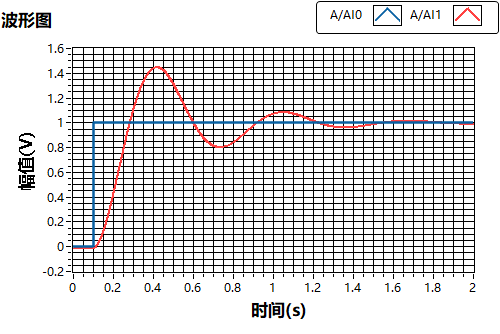
\includegraphics[width=\linewidth]{3.1.png}
\caption{$R=10\ \mathrm{k}\Omega$ 响应曲线}
\end{minipage}
\begin{minipage}{0.48\textwidth}
\centering
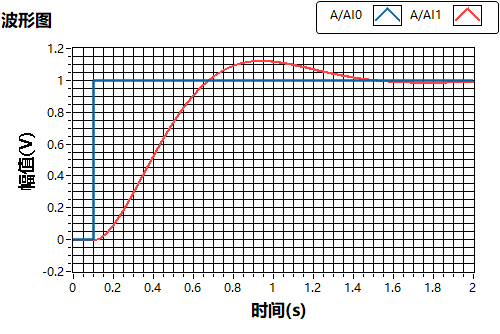
\includegraphics[width=\linewidth]{3.2.png}
\caption{$R=50\ \mathrm{k}\Omega$ 响应曲线}
\end{minipage}
\end{figure}

\begin{figure}[H]
\centering
\begin{minipage}{0.48\textwidth}
\centering
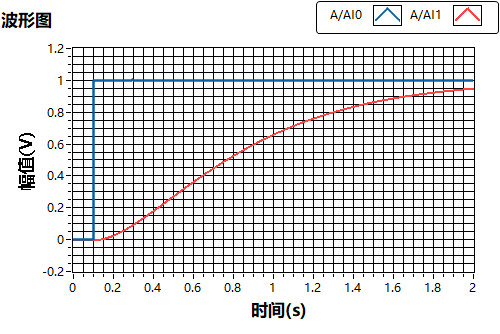
\includegraphics[width=\linewidth]{3.3.png}
\caption{$R=160\ \mathrm{k}\Omega$ 响应曲线}
\end{minipage}
\begin{minipage}{0.48\textwidth}
\centering
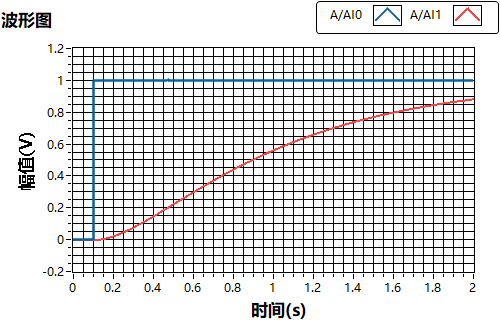
\includegraphics[width=\linewidth]{3.4.png}
\caption{$R=200\ \mathrm{k}\Omega$ 响应曲线}
\end{minipage}
\end{figure}

\vspace{0.5cm}
\textbf{当 $R_0=500\mathrm{k}\Omega$，$C_0=2\mu\mathrm{F}$，$R=10\mathrm{k}\Omega$，$C_1=1\mu\mathrm{F}$，$R_1$ 取 $100\mathrm{k}\Omega$、$200\mathrm{k}\Omega$时，通过观察曲线分析系统性能指标的变化。}

\vspace{0.3cm}
\textbf{答：}
$R_1$ 减小 $\to$ 时间常数 $T_1=R_1C_1$ 减小 $\to$ 无阻尼自然频率 $\omega_n$ 增大、$\xi$ 减小 $\to$ 响应速度加快、超调量增大；
$R_1$ 增大 $\to$ $T_1$ 增大 $\to$ $\omega_n$ 减小、$\xi$ 增大 $\to$ 响应变慢、超调量减小。

\begin{figure}[H]
\centering
\begin{minipage}{0.48\textwidth}
\centering
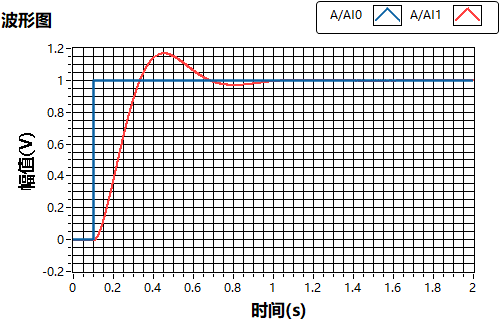
\includegraphics[width=\linewidth]{3.5.png}
\caption{$R_1=100\ \mathrm{k}\Omega$ 响应曲线}
\end{minipage}
\begin{minipage}{0.48\textwidth}
\centering
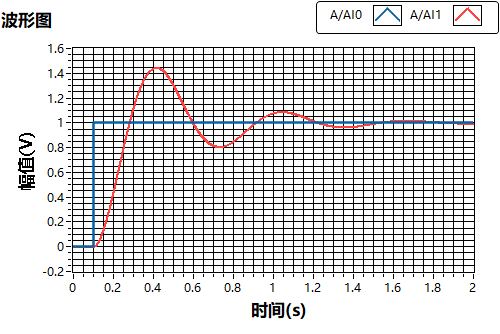
\includegraphics[width=\linewidth]{3.6.png}
\caption{$R_1=200\ \mathrm{k}\Omega$ 响应曲线}
\end{minipage}
\end{figure}

\vspace{0.5cm}
\textbf{分析 $R$ 和 $R_1$ 的变化影响了哪些参量，如何改变系统的动态性能？}

\vspace{0.3cm}
\textbf{答：}
$R$ 主要影响开环增益 $K$，进而改变阻尼比 $\xi$：$R$ 减小使 $K$ 增大、$\xi$ 减小，系统超调量增大、振荡加剧；$R$ 增大使 $K$ 减小、$\xi$ 增大，系统超调量减小、响应变慢。
$R_1$ 主要影响时间常数 $T_1$，进而改变 $\omega_n$ 与 $\xi$：$R_1$ 减小使 $T_1$ 减小、$\omega_n$ 增大、$\xi$ 减小，系统响应速度加快、超调量增大；$R_1$ 增大使 $T_1$ 增大、$\omega_n$ 减小、$\xi$ 增大，系统响应变慢、超调量减小。

\newpage
\subsection{四、实验数据分析}

\subsubsection{1. 实验结果曲线}
\begin{figure}[H]
    \centering
    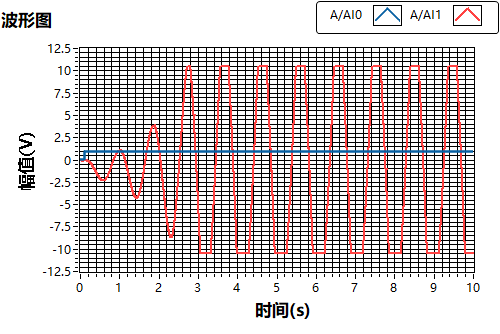
\includegraphics[width=0.8\textwidth]{4.1.png}
    \caption{二阶系统阶跃响应实验曲线}
\end{figure}

\begin{figure}[H]
    \centering
    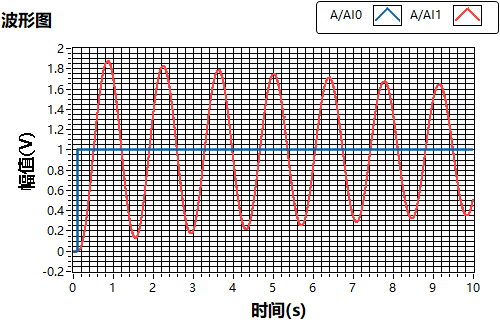
\includegraphics[width=0.8\textwidth]{4.2.png}
    \caption{三阶系统稳定响应曲线}
\end{figure}

\begin{figure}[H]
    \centering
    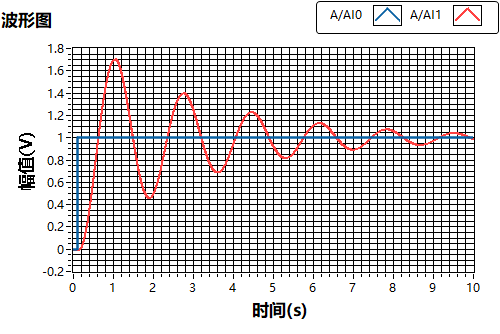
\includegraphics[width=0.8\textwidth]{4.3.png}
    \caption{三阶系统不稳定响应曲线}
\end{figure}

\subsubsection{2. 实验数据表格}
\begin{table}[H]
\centering
\caption{附表1 典型二阶系统瞬态性能指标实验结果I}
\setlength{\tabcolsep}{2pt}
\renewcommand{\arraystretch}{1.6}
\resizebox{\textwidth}{!}{%
\begin{tabular}{|c|c|c|c|c|c|c|c|c|c|c|c|c|c|}
\hline
\multirow{2}{*}{\makecell{$R$\\($\mathrm{k}\Omega$)}} & \multirow{2}{*}{$K$} & \multirow{2}{*}{$\omega_n$} & \multirow{2}{*}{$\xi$} & \multirow{2}{*}{$C(t_p)$} & \multicolumn{2}{c|}{$\delta$ (\%)} & \multicolumn{2}{c|}{$T_p$ (s)} & \multicolumn{2}{c|}{$t_s$ (s)} & \multicolumn{3}{c|}{阶跃响应形式} \\
\cline{6-14}
& & & & & 理论值 & 测量值 & 理论值 & 测量值 & 理论值 & 测量值 & 欠阻尼 & 临界阻尼 & 过阻尼 \\
\hline
10 & 50 & 2.24 & 0.134 & 1.72 & 65.5 & 64.8 & 1.41 & 0.40 & 6.0 & 1.40 & $\surd$ & & \\
\hline
50 & 10 & 2.24 & 0.335 & 1.39 & 33.5 & 34.2 & 1.50 & 0.45 & 4.0 & 1.20 & $\surd$ & & \\
\hline
160 & 3.125 & 2.24 & 0.671 & 1.10 & 6.8 & 7.3 & 1.90 & 0.90 & 3.0 & 1.10 & $\surd$ & & \\
\hline
200 & 2.5 & 2.24 & 0.750 & 1.05 & 2.8 & 0.0 & 2.20 & 2.00 & 3.0 & 1.50 & & & $\surd$ \\
\hline
\end{tabular}%
}
\end{table}

\begin{table}[H]
\centering
\caption{附表2 典型二阶系统瞬态性能指标实验结果II}
\setlength{\tabcolsep}{2pt}
\renewcommand{\arraystretch}{1.6}
\resizebox{\textwidth}{!}{%
\begin{tabular}{|c|c|c|c|c|c|c|c|c|c|c|c|c|c|}
\hline
\multirow{2}{*}{\makecell{$R_1$\\($\mathrm{k}\Omega$)}} & \multirow{2}{*}{$K$} & \multirow{2}{*}{$\omega_n$} & \multirow{2}{*}{$\xi$} & \multirow{2}{*}{$C(t_p)$} & \multicolumn{2}{c|}{$\delta$ (\%)} & \multicolumn{2}{c|}{$T_p$ (s)} & \multicolumn{2}{c|}{$t_s$ (s)} & \multicolumn{3}{c|}{阶跃响应形式} \\
\cline{6-14}
& & & & & 理论值 & 测量值 & 理论值 & 测量值 & 理论值 & 测量值 & 欠阻尼 & 临界阻尼 & 过阻尼 \\
\hline
100 & 50 & 3.16 & 0.530 & 1.20 & 14.0 & 14.8 & 1.10 & 0.40 & 2.5 & 1.00 & $\surd$ & & \\
\hline
200 & 50 & 2.24 & 0.134 & 1.72 & 65.5 & 64.7 & 1.41 & 0.40 & 6.0 & 1.40 & $\surd$ & & \\
\hline
\end{tabular}%
}
\end{table}

\begin{table}[H]
\centering
\caption{附表3 典型三阶系统在不同开环增益下的响应实验结果}
\renewcommand{\arraystretch}{1.4}
\begin{tabular}{|c|c|c|}
\hline $R\ (\mathrm{k}\Omega)$ & 开环增益 $K$ & 稳定性 \\
\hline 10 & 50 & 不稳定 \\
\hline 50 & 10 & 稳定 \\
\hline 100 & 5 & 稳定 \\
\hline 200 & 2.5 & 稳定 \\
\hline
\end{tabular}
\end{table}

\subsubsection{3. 思考题}
\begin{enumerate}[leftmargin=*]
    \item 二阶系统性能分析实验中，改变 $T_1$、$K_1$ 对系统的特征参数 $\xi$，$\omega_n$ 及动态性能指标有何影响。\\
\textbf{答：} $K_1$ 增大会使阻尼比 $\xi$ 减小，超调量 $\delta\%$ 增大，振荡增强；$T_1$ 增大会使 $\omega_n$ 减小，响应变慢，峰值时间和调节时间均增大。

    \item 二阶系统性能分析实验中，若要求减小 $\delta\%$，应采取什么措施？对其他指标有什么影响？\\
\textbf{答：} 增大阻尼比 $\xi$，可减小超调量 $\delta\%$，但会使峰值时间 $T_p$ 和调节时间 $t_s$ 增大，系统响应速度变慢。

    \item 三阶系统的阶跃响应是衰减震荡时，其动态性能在什么情况下可近似等效于其中一对共轭复数极点？\\
\textbf{答：} 当共轭复数极点为主导极点，即实极点远离虚轴、其影响可忽略时，三阶系统可近似由一对共轭复极点表征动态性能。

    \item 分析三阶系统的小惯性环节和大惯性环节，哪个对系统稳定性影响更大？结合实验说明。\\
\textbf{答：} 小惯性环节时间常数小、极点更靠近虚轴，对稳定性影响更大；大惯性环节极点远离虚轴，对系统稳定性影响较小。实验中，当小惯性环节对应增益增大时，系统更易失稳，验证了其对稳定性的主导影响。
\end{enumerate}

\end{document}